% Created by tikzDevice version 0.10.1 on 2017-12-20 13:08:39
% !TEX encoding = UTF-8 Unicode
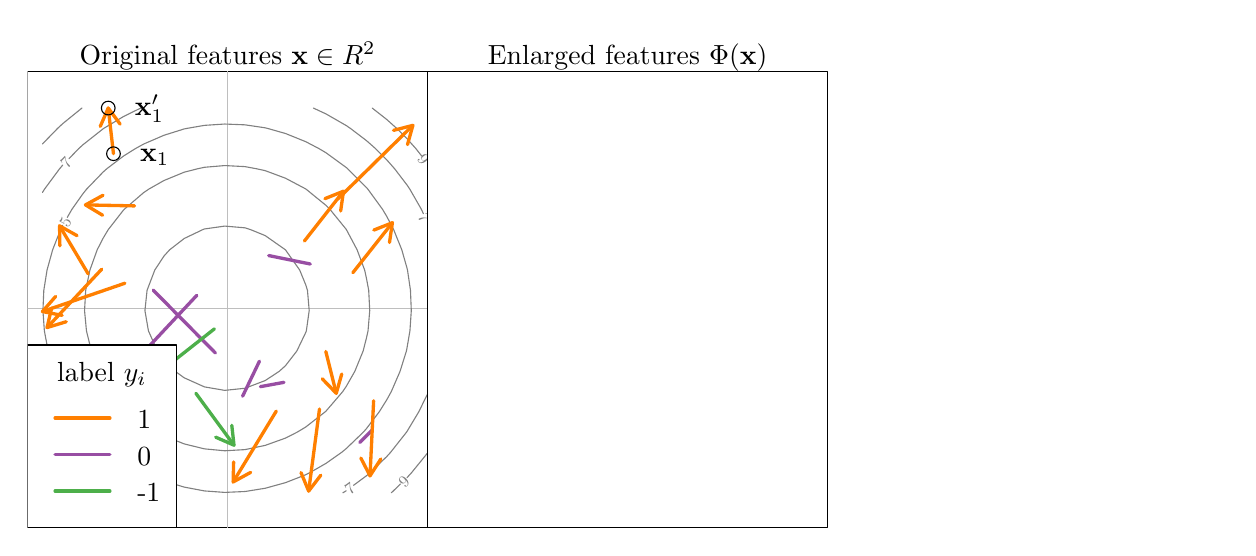
\begin{tikzpicture}[x=1pt,y=1pt]
\definecolor{fillColor}{RGB}{255,255,255}
\path[use as bounding box,fill=fillColor,fill opacity=0.00] (0,0) rectangle (433.62,180.67);
\begin{scope}
\path[clip] (  0.00,  0.00) rectangle (433.62,180.67);
\definecolor{drawColor}{RGB}{0,0,0}

\path[draw=drawColor,line width= 0.4pt,line join=round,line cap=round] (  0.00,  0.00) --
	(144.54,  0.00) --
	(144.54,164.83) --
	(  0.00,164.83) --
	(  0.00,  0.00);
\end{scope}
\begin{scope}
\path[clip] (  0.00,  0.00) rectangle (144.54,164.83);
\definecolor{drawColor}{RGB}{190,190,190}

\path[draw=drawColor,line width= 0.4pt,line join=round,line cap=round] (  0.00, 79.33) -- (144.54, 79.33);

\path[draw=drawColor,line width= 0.4pt,line join=round,line cap=round] ( 72.09,  0.00) -- ( 72.09,164.84);
\end{scope}
\begin{scope}
\path[clip] (  0.00,  0.00) rectangle (433.62,180.67);
\definecolor{drawColor}{RGB}{0,0,0}

\node[text=drawColor,anchor=base,inner sep=0pt, outer sep=0pt, scale=  1.00] at ( 72.27,167.47) {Original features $\mathbf x\in\mathbb R^2$};
\end{scope}
\begin{scope}
\path[clip] (  0.00,  0.00) rectangle (144.54,164.83);
\definecolor{drawColor}{gray}{0.50}

\path[draw=drawColor,line width= 0.4pt,line join=round,line cap=round] ( 46.90, 63.81) --
	( 43.63, 71.13) --
	( 42.37, 78.44) --
	( 43.14, 85.76) --
	( 45.93, 93.08) --
	( 49.26, 98.15) --
	( 51.30,100.40) --
	( 56.57,104.49) --
	( 63.30,107.71) --
	( 63.89,107.93) --
	( 71.21,108.97) --
	( 78.53,108.34) --
	( 80.50,107.71) --
	( 85.84,105.53) --
	( 93.14,100.40) --
	( 93.16,100.38) --
	( 98.30, 93.08) --
	(100.48, 87.74) --
	(101.10, 85.76) --
	(101.73, 78.44) --
	(100.70, 71.13) --
	(100.48, 70.53) --
	( 97.25, 63.81) --
	( 93.16, 58.53) --
	( 90.91, 56.49) --
	( 85.84, 53.16) --
	( 78.53, 50.37) --
	( 71.21, 49.61) --
	( 63.89, 50.86) --
	( 56.57, 54.14) --
	( 53.32, 56.49) --
	( 49.26, 60.55);

\path[draw=drawColor,line width= 0.4pt,line join=round,line cap=round] ( 49.26, 60.55) -- ( 48.82, 61.16);

\node[text=drawColor,rotate=-54.13,anchor=base west,inner sep=0pt, outer sep=0pt, scale=  0.60] at ( 45.07, 62.48) { 1 };

\path[draw=drawColor,line width= 0.4pt,line join=round,line cap=round] ( 27.31, 53.96) --
	( 25.92, 56.49);

\path[draw=drawColor,line width= 0.4pt,line join=round,line cap=round] ( 23.03, 63.81) --
	( 21.24, 71.13) --
	( 20.55, 78.44) --
	( 20.97, 85.76) --
	( 22.49, 93.08) --
	( 25.12,100.40) --
	( 27.31,104.67) --
	( 29.13,107.71) --
	( 34.62,114.76) --
	( 34.88,115.03) --
	( 41.94,121.09) --
	( 43.80,122.35) --
	( 49.26,125.44) --
	( 56.57,128.45) --
	( 61.36,129.67) --
	( 63.89,130.22) --
	( 71.21,130.84) --
	( 78.53,130.46) --
	( 82.78,129.67) --
	( 85.84,129.00) --
	( 93.16,126.27) --
	(100.48,122.40) --
	(100.55,122.35) --
	(107.80,116.45) --
	(109.22,115.03) --
	(115.11,107.79) --
	(115.16,107.71) --
	(119.04,100.40) --
	(121.77, 93.08) --
	(122.43, 90.02) --
	(123.23, 85.76) --
	(123.60, 78.44) --
	(122.99, 71.13) --
	(122.43, 68.59) --
	(121.21, 63.81) --
	(118.21, 56.49) --
	(115.11, 51.04) --
	(113.86, 49.18) --
	(107.80, 42.12) --
	(107.52, 41.86) --
	(100.48, 36.37) --
	( 97.44, 34.54) --
	( 93.16, 32.36) --
	( 85.84, 29.73) --
	( 78.53, 28.20) --
	( 71.21, 27.78) --
	( 63.89, 28.47) --
	( 56.57, 30.26) --
	( 49.26, 33.16) --
	( 46.73, 34.54) --
	( 41.94, 37.63) --
	( 36.79, 41.86) --
	( 34.62, 44.03) --
	( 30.39, 49.18) --
	( 27.31, 53.96);

\path[draw=drawColor,line width= 0.4pt,line join=round,line cap=round] ( 25.92, 56.49) -- ( 24.23, 60.77);

\node[text=drawColor,rotate=-68.44,anchor=base west,inner sep=0pt, outer sep=0pt, scale=  0.60] at ( 20.92, 62.98) { 3 };

\path[draw=drawColor,line width= 0.4pt,line join=round,line cap=round] ( 12.67, 49.26) --
	(  9.63, 56.49) --
	(  7.41, 63.81) --
	(  6.03, 71.13) --
	(  5.51, 78.44) --
	(  5.83, 85.76) --
	(  7.00, 93.08) --
	(  9.02,100.40) --
	( 11.89,107.71) --
	( 12.67,109.25);

\path[draw=drawColor,line width= 0.4pt,line join=round,line cap=round] ( 15.99,115.03) --
	( 19.99,120.69) --
	( 21.33,122.35) --
	( 27.31,128.55) --
	( 28.57,129.67) --
	( 34.62,134.27) --
	( 38.95,136.98) --
	( 41.94,138.63) --
	( 49.26,141.79) --
	( 56.57,144.08) --
	( 57.71,144.30) --
	( 63.89,145.37) --
	( 71.21,145.85) --
	( 78.53,145.56) --
	( 85.84,144.48) --
	( 86.56,144.30) --
	( 93.16,142.43) --
	(100.48,139.47) --
	(105.24,136.98) --
	(107.80,135.47) --
	(115.11,130.14) --
	(115.66,129.67) --
	(122.43,122.89) --
	(122.90,122.35) --
	(128.23,115.03) --
	(129.75,112.48) --
	(132.24,107.71) --
	(135.19,100.40) --
	(137.07, 93.79) --
	(137.25, 93.08) --
	(138.32, 85.76) --
	(138.62, 78.44) --
	(138.13, 71.13) --
	(137.07, 64.94) --
	(136.85, 63.81) --
	(134.56, 56.49) --
	(131.40, 49.18) --
	(129.75, 46.19) --
	(127.04, 41.86) --
	(122.43, 35.81) --
	(121.31, 34.54) --
	(115.11, 28.57) --
	(113.46, 27.22) --
	(107.80, 23.23) --
	(102.02, 19.91) --
	(100.48, 19.12) --
	( 93.16, 16.26) --
	( 85.84, 14.24) --
	( 78.53, 13.06) --
	( 71.21, 12.74) --
	( 63.89, 13.27) --
	( 56.57, 14.65) --
	( 49.26, 16.87) --
	( 42.03, 19.91) --
	( 41.94, 19.95) --
	( 34.62, 24.38) --
	( 30.77, 27.22) --
	( 27.31, 30.17) --
	( 22.93, 34.54) --
	( 19.99, 38.01) --
	( 17.15, 41.86) --
	( 12.71, 49.18) --
	( 12.67, 49.26);

\path[draw=drawColor,line width= 0.4pt,line join=round,line cap=round] ( 14.30,112.09) -- ( 15.99,115.03);

\node[text=drawColor,rotate= 60.15,anchor=base west,inner sep=0pt, outer sep=0pt, scale=  0.60] at ( 14.63,108.13) { 5 };

\path[draw=drawColor,line width= 0.4pt,line join=round,line cap=round] ( 27.31, 14.57) --
	( 20.36, 19.91) --
	( 19.99, 20.23) --
	( 13.00, 27.22) --
	( 12.67, 27.60) --
	(  7.34, 34.54) --
	(  5.35, 37.58);

\path[draw=drawColor,line width= 0.4pt,line join=round,line cap=round] ( 27.61, 14.37) -- ( 27.31, 14.57);

\node[text=drawColor,rotate=-33.12,anchor=base west,inner sep=0pt, outer sep=0pt, scale=  0.60] at ( 26.38, 12.48) { 7 };

\path[draw=drawColor,line width= 0.4pt,line join=round,line cap=round] (  5.35,121.14) --
	(  6.11,122.35) --
	( 11.52,129.67) --
	( 12.67,131.01);

\path[draw=drawColor,line width= 0.4pt,line join=round,line cap=round] ( 18.46,136.98) --
	( 19.99,138.37) --
	( 27.31,144.16) --
	( 27.52,144.30) --
	( 34.62,148.56) --
	( 40.84,151.62);

\path[draw=drawColor,line width= 0.4pt,line join=round,line cap=round] ( 14.94,133.35) -- ( 18.46,136.98);

\node[text=drawColor,rotate= 45.95,anchor=base west,inner sep=0pt, outer sep=0pt, scale=  0.60] at ( 14.30,129.43) { 7 };

\path[draw=drawColor,line width= 0.4pt,line join=round,line cap=round] (142.26,115.03) --
	(138.07,122.35) --
	(137.07,123.82) --
	(132.61,129.67) --
	(129.75,132.92) --
	(125.69,136.98) --
	(122.43,139.85) --
	(116.58,144.30) --
	(115.11,145.30) --
	(107.80,149.50) --
	(103.25,151.62);

\path[draw=drawColor,line width= 0.4pt,line join=round,line cap=round] (143.00,113.45) -- (142.26,115.03);

\node[text=drawColor,rotate=-65.00,anchor=base west,inner sep=0pt, outer sep=0pt, scale=  0.60] at (140.95,112.49) { 7 };

\path[draw=drawColor,line width= 0.4pt,line join=round,line cap=round] (113.90, 12.59) --
	(115.11, 13.34);

\path[draw=drawColor,line width= 0.4pt,line join=round,line cap=round] (122.43, 18.76) --
	(123.77, 19.91) --
	(129.75, 25.69) --
	(131.14, 27.22) --
	(136.92, 34.54) --
	(137.07, 34.76) --
	(141.32, 41.86) --
	(144.38, 48.07);

\path[draw=drawColor,line width= 0.4pt,line join=round,line cap=round] (117.74, 15.29) -- (122.43, 18.76);

\node[text=drawColor,rotate= 36.52,anchor=base west,inner sep=0pt, outer sep=0pt, scale=  0.60] at (116.46, 11.53) { 7 };

\path[draw=drawColor,line width= 0.4pt,line join=round,line cap=round] ( 12.68, 12.59) --
	( 12.67, 12.60) --
	(  5.36, 19.91) --
	(  5.35, 19.92);

\path[draw=drawColor,line width= 0.4pt,line join=round,line cap=round] (  5.35,138.66) --
	( 10.84,144.30) --
	( 12.67,145.99) --
	( 19.60,151.62);

\path[draw=drawColor,line width= 0.4pt,line join=round,line cap=round] (140.26,136.98) --
	(137.07,140.56) --
	(133.32,144.30) --
	(129.75,147.49) --
	(124.50,151.62);

\path[draw=drawColor,line width= 0.4pt,line join=round,line cap=round] (142.36,134.31) -- (140.26,136.98);

\node[text=drawColor,rotate=-51.83,anchor=base west,inner sep=0pt, outer sep=0pt, scale=  0.60] at (140.58,132.91) { 9 };

\path[draw=drawColor,line width= 0.4pt,line join=round,line cap=round] (137.07, 18.07) --
	(138.75, 19.91) --
	(144.38, 26.84);

\path[draw=drawColor,line width= 0.4pt,line join=round,line cap=round] (131.42, 12.59) -- (134.72, 15.80);

\node[text=drawColor,rotate= 44.21,anchor=base west,inner sep=0pt, outer sep=0pt, scale=  0.60] at (136.30, 14.17) { 9 };
\definecolor{drawColor}{RGB}{152,78,163}

\path[draw=drawColor,line width= 1.2pt,line join=round,line cap=round] ( 61.12, 83.95) -- ( 43.66, 65.31);

\path[draw=drawColor,line width= 1.2pt,line join=round,line cap=round] ( 84.09, 50.95) -- ( 92.61, 52.51);

\path[draw=drawColor,line width= 1.2pt,line join=round,line cap=round] (120.03, 30.80) -- (124.47, 35.29);

\path[draw=drawColor,line width= 1.2pt,line join=round,line cap=round] (102.12, 95.27) -- ( 87.09, 98.32);

\path[draw=drawColor,line width= 1.2pt,line join=round,line cap=round] ( 45.37, 85.82) -- ( 67.82, 63.12);

\path[draw=drawColor,line width= 1.2pt,line join=round,line cap=round] ( 77.66, 47.49) -- ( 83.75, 60.15);
\definecolor{drawColor}{RGB}{255,127,0}

\path[draw=drawColor,line width= 1.2pt,line join=round,line cap=round] ( 31.00,135.13) -- ( 29.11,151.62);

\path[draw=drawColor,line width= 1.2pt,line join=round,line cap=round] ( 33.41,145.81) --
	( 29.11,151.62) --
	( 26.23,144.99);

\path[draw=drawColor,line width= 1.2pt,line join=round,line cap=round] (105.45, 42.87) -- (101.53, 13.22);

\path[draw=drawColor,line width= 1.2pt,line join=round,line cap=round] ( 98.77, 19.90) --
	(101.53, 13.22) --
	(105.93, 18.95);

\path[draw=drawColor,line width= 1.2pt,line join=round,line cap=round] (111.97,118.65) -- (139.19,145.37);

\path[draw=drawColor,line width= 1.2pt,line join=round,line cap=round] (137.25,138.41) --
	(139.19,145.37) --
	(132.19,143.56);

\path[draw=drawColor,line width= 1.2pt,line join=round,line cap=round] (117.50, 92.13) -- (131.79,110.19);

\path[draw=drawColor,line width= 1.2pt,line join=round,line cap=round] (130.74,103.04) --
	(131.79,110.19) --
	(125.08,107.53);

\path[draw=drawColor,line width= 1.2pt,line join=round,line cap=round] (125.01, 45.85) -- (123.70, 18.73);

\path[draw=drawColor,line width= 1.2pt,line join=round,line cap=round] (120.40, 25.15) --
	(123.70, 18.73) --
	(127.62, 24.80);

\path[draw=drawColor,line width= 1.2pt,line join=round,line cap=round] (107.73, 63.64) -- (111.50, 48.56);

\path[draw=drawColor,line width= 1.2pt,line join=round,line cap=round] (106.47, 53.76) --
	(111.50, 48.56) --
	(113.49, 55.51);

\path[draw=drawColor,line width= 1.2pt,line join=round,line cap=round] (100.01,103.59) -- (114.12,121.57);

\path[draw=drawColor,line width= 1.2pt,line join=round,line cap=round] (113.10,114.42) --
	(114.12,121.57) --
	(107.41,118.88);

\path[draw=drawColor,line width= 1.2pt,line join=round,line cap=round] ( 89.83, 42.11) -- ( 74.25, 16.51);

\path[draw=drawColor,line width= 1.2pt,line join=round,line cap=round] ( 74.42, 23.74) --
	( 74.25, 16.51) --
	( 80.59, 19.98);

\path[draw=drawColor,line width= 1.2pt,line join=round,line cap=round] ( 26.76, 93.40) -- (  7.01, 72.31);

\path[draw=drawColor,line width= 1.2pt,line join=round,line cap=round] (  8.65, 79.35) --
	(  7.01, 72.31) --
	( 13.93, 74.41);

\path[draw=drawColor,line width= 1.2pt,line join=round,line cap=round] ( 35.13, 88.32) -- (  5.35, 78.10);

\path[draw=drawColor,line width= 1.2pt,line join=round,line cap=round] ( 10.10, 83.55) --
	(  5.35, 78.10) --
	( 12.45, 76.71);

\path[draw=drawColor,line width= 1.2pt,line join=round,line cap=round] ( 21.85, 91.74) -- ( 11.53,109.04);

\path[draw=drawColor,line width= 1.2pt,line join=round,line cap=round] ( 17.84,105.52) --
	( 11.53,109.04) --
	( 11.63,101.81);

\path[draw=drawColor,line width= 1.2pt,line join=round,line cap=round] ( 38.60,116.27) -- ( 20.89,116.63);

\path[draw=drawColor,line width= 1.2pt,line join=round,line cap=round] ( 27.23,120.11) --
	( 20.89,116.63) --
	( 27.08,112.89);
\definecolor{drawColor}{RGB}{77,175,74}

\path[draw=drawColor,line width= 1.2pt,line join=round,line cap=round] ( 67.47, 71.83) -- ( 40.49, 50.57);

\path[draw=drawColor,line width= 1.2pt,line join=round,line cap=round] ( 43.17, 57.28) --
	( 40.49, 50.57) --
	( 47.65, 51.61);

\path[draw=drawColor,line width= 1.2pt,line join=round,line cap=round] ( 60.78, 48.55) -- ( 74.55, 29.80);

\path[draw=drawColor,line width= 1.2pt,line join=round,line cap=round] ( 67.94, 32.70) --
	( 74.55, 29.80) --
	( 73.76, 36.98);
\definecolor{drawColor}{RGB}{0,0,0}
\definecolor{fillColor}{RGB}{255,255,255}

\path[draw=drawColor,line width= 0.4pt,line join=round,line cap=round,fill=fillColor] (  0.00, 66.00) rectangle ( 53.62,  0.00);
\definecolor{drawColor}{RGB}{255,127,0}

\path[draw=drawColor,line width= 1.2pt,line join=round,line cap=round] (  9.90, 39.60) -- ( 29.70, 39.60);
\definecolor{drawColor}{RGB}{152,78,163}

\path[draw=drawColor,line width= 1.2pt,line join=round,line cap=round] (  9.90, 26.40) -- ( 29.70, 26.40);
\definecolor{drawColor}{RGB}{77,175,74}

\path[draw=drawColor,line width= 1.2pt,line join=round,line cap=round] (  9.90, 13.20) -- ( 29.70, 13.20);
\definecolor{drawColor}{RGB}{0,0,0}

\node[text=drawColor,anchor=base,inner sep=0pt, outer sep=0pt, scale=  1.00] at ( 26.81, 52.80) {label $y_i$};

\node[text=drawColor,anchor=base west,inner sep=0pt, outer sep=0pt, scale=  1.00] at ( 39.60, 35.83) {1};

\node[text=drawColor,anchor=base west,inner sep=0pt, outer sep=0pt, scale=  1.00] at ( 39.60, 22.63) {0};

\node[text=drawColor,anchor=base west,inner sep=0pt, outer sep=0pt, scale=  1.00] at ( 39.60,  9.43) {-1};

\path[draw=drawColor,line width= 0.4pt,line join=round,line cap=round] ( 31.00,135.13) circle (  2.47);

\path[draw=drawColor,line width= 0.4pt,line join=round,line cap=round] ( 29.11,151.62) circle (  2.47);

\node[text=drawColor,anchor=base,inner sep=0pt, outer sep=0pt, scale=  1.00] at ( 45.89,132.39) {$\mathbf x_{1}$};

\node[text=drawColor,anchor=base,inner sep=0pt, outer sep=0pt, scale=  1.00] at ( 44.00,148.88) {$\mathbf x_{1}'$};
\end{scope}
\begin{scope}
\path[clip] (  0.00,  0.00) rectangle (433.62,180.67);
\definecolor{drawColor}{RGB}{0,0,0}

\path[draw=drawColor,line width= 0.4pt,line join=round,line cap=round] (144.54,  0.00) --
	(289.08,  0.00) --
	(289.08,164.83) --
	(144.54,164.83) --
	(144.54,  0.00);
\end{scope}
\begin{scope}
\path[clip] (  0.00,  0.00) rectangle (433.62,180.67);
\definecolor{drawColor}{RGB}{0,0,0}

\node[text=drawColor,anchor=base,inner sep=0pt, outer sep=0pt, scale=  1.00] at (216.81,167.47) {Enlarged features $\Phi(\mathbf x)$};
\end{scope}
\end{tikzpicture}
\begin{tikzpicture}[x=1pt,y=1pt]
\definecolor{fillColor}{RGB}{255,255,255}
\path[use as bounding box,fill=fillColor,fill opacity=0.00] (0,0) rectangle (433.62,180.67);
\begin{scope}
\path[clip] (  0.00,  0.00) rectangle (433.62,180.67);
\definecolor{drawColor}{RGB}{0,0,0}

\path[draw=drawColor,line width= 0.4pt,line join=round,line cap=round] (  0.00,  0.00) --
	(144.54,  0.00) --
	(144.54,164.83) --
	(  0.00,164.83) --
	(  0.00,  0.00);
\end{scope}
\begin{scope}
\path[clip] (  0.00,  0.00) rectangle (144.54,164.83);
\definecolor{drawColor}{RGB}{190,190,190}

\path[draw=drawColor,line width= 0.4pt,line join=round,line cap=round] (  0.00, 79.33) -- (144.54, 79.33);

\path[draw=drawColor,line width= 0.4pt,line join=round,line cap=round] ( 72.09,  0.00) -- ( 72.09,164.84);
\end{scope}
\begin{scope}
\path[clip] (  0.00,  0.00) rectangle (433.62,180.67);
\definecolor{drawColor}{RGB}{0,0,0}

\node[text=drawColor,anchor=base,inner sep=0pt, outer sep=0pt, scale=  1.00] at ( 72.27,167.47) {Original features $\mathbf x\in\mathbb R^2$};
\end{scope}
\begin{scope}
\path[clip] (  0.00,  0.00) rectangle (144.54,164.83);
\definecolor{drawColor}{gray}{0.50}

\path[draw=drawColor,line width= 0.4pt,line join=round,line cap=round] ( 46.90, 63.81) --
	( 43.63, 71.13) --
	( 42.37, 78.44) --
	( 43.14, 85.76) --
	( 45.93, 93.08) --
	( 49.26, 98.15) --
	( 51.30,100.40) --
	( 56.57,104.49) --
	( 63.30,107.71) --
	( 63.89,107.93) --
	( 71.21,108.97) --
	( 78.53,108.34) --
	( 80.50,107.71) --
	( 85.84,105.53) --
	( 93.14,100.40) --
	( 93.16,100.38) --
	( 98.30, 93.08) --
	(100.48, 87.74) --
	(101.10, 85.76) --
	(101.73, 78.44) --
	(100.70, 71.13) --
	(100.48, 70.53) --
	( 97.25, 63.81) --
	( 93.16, 58.53) --
	( 90.91, 56.49) --
	( 85.84, 53.16) --
	( 78.53, 50.37) --
	( 71.21, 49.61) --
	( 63.89, 50.86) --
	( 56.57, 54.14) --
	( 53.32, 56.49) --
	( 49.26, 60.55);

\path[draw=drawColor,line width= 0.4pt,line join=round,line cap=round] ( 49.26, 60.55) -- ( 48.82, 61.16);

\node[text=drawColor,rotate=-54.13,anchor=base west,inner sep=0pt, outer sep=0pt, scale=  0.60] at ( 45.07, 62.48) { 1 };

\path[draw=drawColor,line width= 0.4pt,line join=round,line cap=round] ( 27.31, 53.96) --
	( 25.92, 56.49);

\path[draw=drawColor,line width= 0.4pt,line join=round,line cap=round] ( 23.03, 63.81) --
	( 21.24, 71.13) --
	( 20.55, 78.44) --
	( 20.97, 85.76) --
	( 22.49, 93.08) --
	( 25.12,100.40) --
	( 27.31,104.67) --
	( 29.13,107.71) --
	( 34.62,114.76) --
	( 34.88,115.03) --
	( 41.94,121.09) --
	( 43.80,122.35) --
	( 49.26,125.44) --
	( 56.57,128.45) --
	( 61.36,129.67) --
	( 63.89,130.22) --
	( 71.21,130.84) --
	( 78.53,130.46) --
	( 82.78,129.67) --
	( 85.84,129.00) --
	( 93.16,126.27) --
	(100.48,122.40) --
	(100.55,122.35) --
	(107.80,116.45) --
	(109.22,115.03) --
	(115.11,107.79) --
	(115.16,107.71) --
	(119.04,100.40) --
	(121.77, 93.08) --
	(122.43, 90.02) --
	(123.23, 85.76) --
	(123.60, 78.44) --
	(122.99, 71.13) --
	(122.43, 68.59) --
	(121.21, 63.81) --
	(118.21, 56.49) --
	(115.11, 51.04) --
	(113.86, 49.18) --
	(107.80, 42.12) --
	(107.52, 41.86) --
	(100.48, 36.37) --
	( 97.44, 34.54) --
	( 93.16, 32.36) --
	( 85.84, 29.73) --
	( 78.53, 28.20) --
	( 71.21, 27.78) --
	( 63.89, 28.47) --
	( 56.57, 30.26) --
	( 49.26, 33.16) --
	( 46.73, 34.54) --
	( 41.94, 37.63) --
	( 36.79, 41.86) --
	( 34.62, 44.03) --
	( 30.39, 49.18) --
	( 27.31, 53.96);

\path[draw=drawColor,line width= 0.4pt,line join=round,line cap=round] ( 25.92, 56.49) -- ( 24.23, 60.77);

\node[text=drawColor,rotate=-68.44,anchor=base west,inner sep=0pt, outer sep=0pt, scale=  0.60] at ( 20.92, 62.98) { 3 };

\path[draw=drawColor,line width= 0.4pt,line join=round,line cap=round] ( 12.67, 49.26) --
	(  9.63, 56.49) --
	(  7.41, 63.81) --
	(  6.03, 71.13) --
	(  5.51, 78.44) --
	(  5.83, 85.76) --
	(  7.00, 93.08) --
	(  9.02,100.40) --
	( 11.89,107.71) --
	( 12.67,109.25);

\path[draw=drawColor,line width= 0.4pt,line join=round,line cap=round] ( 15.99,115.03) --
	( 19.99,120.69) --
	( 21.33,122.35) --
	( 27.31,128.55) --
	( 28.57,129.67) --
	( 34.62,134.27) --
	( 38.95,136.98) --
	( 41.94,138.63) --
	( 49.26,141.79) --
	( 56.57,144.08) --
	( 57.71,144.30) --
	( 63.89,145.37) --
	( 71.21,145.85) --
	( 78.53,145.56) --
	( 85.84,144.48) --
	( 86.56,144.30) --
	( 93.16,142.43) --
	(100.48,139.47) --
	(105.24,136.98) --
	(107.80,135.47) --
	(115.11,130.14) --
	(115.66,129.67) --
	(122.43,122.89) --
	(122.90,122.35) --
	(128.23,115.03) --
	(129.75,112.48) --
	(132.24,107.71) --
	(135.19,100.40) --
	(137.07, 93.79) --
	(137.25, 93.08) --
	(138.32, 85.76) --
	(138.62, 78.44) --
	(138.13, 71.13) --
	(137.07, 64.94) --
	(136.85, 63.81) --
	(134.56, 56.49) --
	(131.40, 49.18) --
	(129.75, 46.19) --
	(127.04, 41.86) --
	(122.43, 35.81) --
	(121.31, 34.54) --
	(115.11, 28.57) --
	(113.46, 27.22) --
	(107.80, 23.23) --
	(102.02, 19.91) --
	(100.48, 19.12) --
	( 93.16, 16.26) --
	( 85.84, 14.24) --
	( 78.53, 13.06) --
	( 71.21, 12.74) --
	( 63.89, 13.27) --
	( 56.57, 14.65) --
	( 49.26, 16.87) --
	( 42.03, 19.91) --
	( 41.94, 19.95) --
	( 34.62, 24.38) --
	( 30.77, 27.22) --
	( 27.31, 30.17) --
	( 22.93, 34.54) --
	( 19.99, 38.01) --
	( 17.15, 41.86) --
	( 12.71, 49.18) --
	( 12.67, 49.26);

\path[draw=drawColor,line width= 0.4pt,line join=round,line cap=round] ( 14.30,112.09) -- ( 15.99,115.03);

\node[text=drawColor,rotate= 60.15,anchor=base west,inner sep=0pt, outer sep=0pt, scale=  0.60] at ( 14.63,108.13) { 5 };

\path[draw=drawColor,line width= 0.4pt,line join=round,line cap=round] ( 27.31, 14.57) --
	( 20.36, 19.91) --
	( 19.99, 20.23) --
	( 13.00, 27.22) --
	( 12.67, 27.60) --
	(  7.34, 34.54) --
	(  5.35, 37.58);

\path[draw=drawColor,line width= 0.4pt,line join=round,line cap=round] ( 27.61, 14.37) -- ( 27.31, 14.57);

\node[text=drawColor,rotate=-33.12,anchor=base west,inner sep=0pt, outer sep=0pt, scale=  0.60] at ( 26.38, 12.48) { 7 };

\path[draw=drawColor,line width= 0.4pt,line join=round,line cap=round] (  5.35,121.14) --
	(  6.11,122.35) --
	( 11.52,129.67) --
	( 12.67,131.01);

\path[draw=drawColor,line width= 0.4pt,line join=round,line cap=round] ( 18.46,136.98) --
	( 19.99,138.37) --
	( 27.31,144.16) --
	( 27.52,144.30) --
	( 34.62,148.56) --
	( 40.84,151.62);

\path[draw=drawColor,line width= 0.4pt,line join=round,line cap=round] ( 14.94,133.35) -- ( 18.46,136.98);

\node[text=drawColor,rotate= 45.95,anchor=base west,inner sep=0pt, outer sep=0pt, scale=  0.60] at ( 14.30,129.43) { 7 };

\path[draw=drawColor,line width= 0.4pt,line join=round,line cap=round] (142.26,115.03) --
	(138.07,122.35) --
	(137.07,123.82) --
	(132.61,129.67) --
	(129.75,132.92) --
	(125.69,136.98) --
	(122.43,139.85) --
	(116.58,144.30) --
	(115.11,145.30) --
	(107.80,149.50) --
	(103.25,151.62);

\path[draw=drawColor,line width= 0.4pt,line join=round,line cap=round] (143.00,113.45) -- (142.26,115.03);

\node[text=drawColor,rotate=-65.00,anchor=base west,inner sep=0pt, outer sep=0pt, scale=  0.60] at (140.95,112.49) { 7 };

\path[draw=drawColor,line width= 0.4pt,line join=round,line cap=round] (113.90, 12.59) --
	(115.11, 13.34);

\path[draw=drawColor,line width= 0.4pt,line join=round,line cap=round] (122.43, 18.76) --
	(123.77, 19.91) --
	(129.75, 25.69) --
	(131.14, 27.22) --
	(136.92, 34.54) --
	(137.07, 34.76) --
	(141.32, 41.86) --
	(144.38, 48.07);

\path[draw=drawColor,line width= 0.4pt,line join=round,line cap=round] (117.74, 15.29) -- (122.43, 18.76);

\node[text=drawColor,rotate= 36.52,anchor=base west,inner sep=0pt, outer sep=0pt, scale=  0.60] at (116.46, 11.53) { 7 };

\path[draw=drawColor,line width= 0.4pt,line join=round,line cap=round] ( 12.68, 12.59) --
	( 12.67, 12.60) --
	(  5.36, 19.91) --
	(  5.35, 19.92);

\path[draw=drawColor,line width= 0.4pt,line join=round,line cap=round] (  5.35,138.66) --
	( 10.84,144.30) --
	( 12.67,145.99) --
	( 19.60,151.62);

\path[draw=drawColor,line width= 0.4pt,line join=round,line cap=round] (140.26,136.98) --
	(137.07,140.56) --
	(133.32,144.30) --
	(129.75,147.49) --
	(124.50,151.62);

\path[draw=drawColor,line width= 0.4pt,line join=round,line cap=round] (142.36,134.31) -- (140.26,136.98);

\node[text=drawColor,rotate=-51.83,anchor=base west,inner sep=0pt, outer sep=0pt, scale=  0.60] at (140.58,132.91) { 9 };

\path[draw=drawColor,line width= 0.4pt,line join=round,line cap=round] (137.07, 18.07) --
	(138.75, 19.91) --
	(144.38, 26.84);

\path[draw=drawColor,line width= 0.4pt,line join=round,line cap=round] (131.42, 12.59) -- (134.72, 15.80);

\node[text=drawColor,rotate= 44.21,anchor=base west,inner sep=0pt, outer sep=0pt, scale=  0.60] at (136.30, 14.17) { 9 };
\definecolor{drawColor}{RGB}{152,78,163}

\path[draw=drawColor,line width= 1.2pt,line join=round,line cap=round] ( 61.12, 83.95) -- ( 43.66, 65.31);

\path[draw=drawColor,line width= 1.2pt,line join=round,line cap=round] ( 84.09, 50.95) -- ( 92.61, 52.51);

\path[draw=drawColor,line width= 1.2pt,line join=round,line cap=round] (120.03, 30.80) -- (124.47, 35.29);

\path[draw=drawColor,line width= 1.2pt,line join=round,line cap=round] (102.12, 95.27) -- ( 87.09, 98.32);

\path[draw=drawColor,line width= 1.2pt,line join=round,line cap=round] ( 45.37, 85.82) -- ( 67.82, 63.12);

\path[draw=drawColor,line width= 1.2pt,line join=round,line cap=round] ( 77.66, 47.49) -- ( 83.75, 60.15);
\definecolor{drawColor}{RGB}{255,127,0}

\path[draw=drawColor,line width= 1.2pt,line join=round,line cap=round] ( 31.00,135.13) -- ( 29.11,151.62);

\path[draw=drawColor,line width= 1.2pt,line join=round,line cap=round] ( 33.41,145.81) --
	( 29.11,151.62) --
	( 26.23,144.99);

\path[draw=drawColor,line width= 1.2pt,line join=round,line cap=round] (105.45, 42.87) -- (101.53, 13.22);

\path[draw=drawColor,line width= 1.2pt,line join=round,line cap=round] ( 98.77, 19.90) --
	(101.53, 13.22) --
	(105.93, 18.95);

\path[draw=drawColor,line width= 1.2pt,line join=round,line cap=round] (111.97,118.65) -- (139.19,145.37);

\path[draw=drawColor,line width= 1.2pt,line join=round,line cap=round] (137.25,138.41) --
	(139.19,145.37) --
	(132.19,143.56);

\path[draw=drawColor,line width= 1.2pt,line join=round,line cap=round] (117.50, 92.13) -- (131.79,110.19);

\path[draw=drawColor,line width= 1.2pt,line join=round,line cap=round] (130.74,103.04) --
	(131.79,110.19) --
	(125.08,107.53);

\path[draw=drawColor,line width= 1.2pt,line join=round,line cap=round] (125.01, 45.85) -- (123.70, 18.73);

\path[draw=drawColor,line width= 1.2pt,line join=round,line cap=round] (120.40, 25.15) --
	(123.70, 18.73) --
	(127.62, 24.80);

\path[draw=drawColor,line width= 1.2pt,line join=round,line cap=round] (107.73, 63.64) -- (111.50, 48.56);

\path[draw=drawColor,line width= 1.2pt,line join=round,line cap=round] (106.47, 53.76) --
	(111.50, 48.56) --
	(113.49, 55.51);

\path[draw=drawColor,line width= 1.2pt,line join=round,line cap=round] (100.01,103.59) -- (114.12,121.57);

\path[draw=drawColor,line width= 1.2pt,line join=round,line cap=round] (113.10,114.42) --
	(114.12,121.57) --
	(107.41,118.88);

\path[draw=drawColor,line width= 1.2pt,line join=round,line cap=round] ( 89.83, 42.11) -- ( 74.25, 16.51);

\path[draw=drawColor,line width= 1.2pt,line join=round,line cap=round] ( 74.42, 23.74) --
	( 74.25, 16.51) --
	( 80.59, 19.98);

\path[draw=drawColor,line width= 1.2pt,line join=round,line cap=round] ( 26.76, 93.40) -- (  7.01, 72.31);

\path[draw=drawColor,line width= 1.2pt,line join=round,line cap=round] (  8.65, 79.35) --
	(  7.01, 72.31) --
	( 13.93, 74.41);

\path[draw=drawColor,line width= 1.2pt,line join=round,line cap=round] ( 35.13, 88.32) -- (  5.35, 78.10);

\path[draw=drawColor,line width= 1.2pt,line join=round,line cap=round] ( 10.10, 83.55) --
	(  5.35, 78.10) --
	( 12.45, 76.71);

\path[draw=drawColor,line width= 1.2pt,line join=round,line cap=round] ( 21.85, 91.74) -- ( 11.53,109.04);

\path[draw=drawColor,line width= 1.2pt,line join=round,line cap=round] ( 17.84,105.52) --
	( 11.53,109.04) --
	( 11.63,101.81);

\path[draw=drawColor,line width= 1.2pt,line join=round,line cap=round] ( 38.60,116.27) -- ( 20.89,116.63);

\path[draw=drawColor,line width= 1.2pt,line join=round,line cap=round] ( 27.23,120.11) --
	( 20.89,116.63) --
	( 27.08,112.89);
\definecolor{drawColor}{RGB}{77,175,74}

\path[draw=drawColor,line width= 1.2pt,line join=round,line cap=round] ( 67.47, 71.83) -- ( 40.49, 50.57);

\path[draw=drawColor,line width= 1.2pt,line join=round,line cap=round] ( 43.17, 57.28) --
	( 40.49, 50.57) --
	( 47.65, 51.61);

\path[draw=drawColor,line width= 1.2pt,line join=round,line cap=round] ( 60.78, 48.55) -- ( 74.55, 29.80);

\path[draw=drawColor,line width= 1.2pt,line join=round,line cap=round] ( 67.94, 32.70) --
	( 74.55, 29.80) --
	( 73.76, 36.98);
\definecolor{drawColor}{RGB}{0,0,0}
\definecolor{fillColor}{RGB}{255,255,255}

\path[draw=drawColor,line width= 0.4pt,line join=round,line cap=round,fill=fillColor] (  0.00, 66.00) rectangle ( 53.62,  0.00);
\definecolor{drawColor}{RGB}{255,127,0}

\path[draw=drawColor,line width= 1.2pt,line join=round,line cap=round] (  9.90, 39.60) -- ( 29.70, 39.60);
\definecolor{drawColor}{RGB}{152,78,163}

\path[draw=drawColor,line width= 1.2pt,line join=round,line cap=round] (  9.90, 26.40) -- ( 29.70, 26.40);
\definecolor{drawColor}{RGB}{77,175,74}

\path[draw=drawColor,line width= 1.2pt,line join=round,line cap=round] (  9.90, 13.20) -- ( 29.70, 13.20);
\definecolor{drawColor}{RGB}{0,0,0}

\node[text=drawColor,anchor=base,inner sep=0pt, outer sep=0pt, scale=  1.00] at ( 26.81, 52.80) {label $y_i$};

\node[text=drawColor,anchor=base west,inner sep=0pt, outer sep=0pt, scale=  1.00] at ( 39.60, 35.83) {1};

\node[text=drawColor,anchor=base west,inner sep=0pt, outer sep=0pt, scale=  1.00] at ( 39.60, 22.63) {0};

\node[text=drawColor,anchor=base west,inner sep=0pt, outer sep=0pt, scale=  1.00] at ( 39.60,  9.43) {-1};

\path[draw=drawColor,line width= 0.4pt,line join=round,line cap=round] ( 31.00,135.13) circle (  2.47);

\path[draw=drawColor,line width= 0.4pt,line join=round,line cap=round] ( 29.11,151.62) circle (  2.47);

\node[text=drawColor,anchor=base,inner sep=0pt, outer sep=0pt, scale=  1.00] at ( 45.89,132.39) {$\mathbf x_{1}$};

\node[text=drawColor,anchor=base,inner sep=0pt, outer sep=0pt, scale=  1.00] at ( 44.00,148.88) {$\mathbf x_{1}'$};
\end{scope}
\begin{scope}
\path[clip] (  0.00,  0.00) rectangle (433.62,180.67);
\definecolor{drawColor}{RGB}{0,0,0}

\path[draw=drawColor,line width= 0.4pt,line join=round,line cap=round] (144.54,  0.00) --
	(289.08,  0.00) --
	(289.08,164.83) --
	(144.54,164.83) --
	(144.54,  0.00);
\end{scope}
\begin{scope}
\path[clip] (  0.00,  0.00) rectangle (433.62,180.67);
\definecolor{drawColor}{RGB}{0,0,0}

\node[text=drawColor,anchor=base,inner sep=0pt, outer sep=0pt, scale=  1.00] at (216.81,167.47) {Enlarged features $\Phi(\mathbf x)$};
\end{scope}
\begin{scope}
\path[clip] (144.54,  0.00) rectangle (289.08,164.83);
\definecolor{drawColor}{gray}{0.50}

\node[text=drawColor,rotate=-45.00,anchor=base,inner sep=0pt, outer sep=0pt, scale=  0.80] at (259.58, 62.82) {$r(\mathbf x)=\mathbf w^\intercal \Phi(\mathbf x)$};

\path[draw=drawColor,line width= 0.4pt,line join=round,line cap=round] (176.86,  6.10) --
	(175.13,  7.83) --
	(168.82, 14.14) --
	(167.10, 15.87);

\path[draw=drawColor,line width= 0.4pt,line join=round,line cap=round] (160.79, 22.17) --
	(159.06, 23.90) --
	(152.76, 30.20) --
	(151.03, 31.93);

\path[draw=drawColor,line width= 0.4pt,line join=round,line cap=round] (164.79, 18.18) -- (160.79, 22.17);

\node[text=drawColor,rotate=-45.02,anchor=base west,inner sep=0pt, outer sep=0pt, scale=  0.60] at (163.19, 16.58) { 1 };

\path[draw=drawColor,line width= 0.4pt,line join=round,line cap=round] (199.23,  9.65) --
	(194.74, 14.14) --
	(191.19, 17.68) --
	(186.71, 22.17) --
	(183.16, 25.72) --
	(178.67, 30.20) --
	(175.13, 33.75) --
	(170.64, 38.24) --
	(167.10, 41.78) --
	(162.61, 46.27) --
	(159.06, 49.81) --
	(154.58, 54.30) --
	(151.03, 57.85);

\path[draw=drawColor,line width= 0.4pt,line join=round,line cap=round] (200.46,  8.41) -- (199.23,  9.65);

\node[text=drawColor,rotate=-45.02,anchor=base west,inner sep=0pt, outer sep=0pt, scale=  0.60] at (198.86,  6.82) { 2 };

\path[draw=drawColor,line width= 0.4pt,line join=round,line cap=round] (228.69,  6.10) --
	(223.33, 11.47);

\path[draw=drawColor,line width= 0.4pt,line join=round,line cap=round] (220.65, 14.14) --
	(215.29, 19.50) --
	(212.62, 22.17) --
	(207.26, 27.53) --
	(204.59, 30.20) --
	(199.23, 35.56) --
	(196.56, 38.24) --
	(191.19, 43.60) --
	(188.52, 46.27) --
	(183.16, 51.63) --
	(180.49, 54.30) --
	(175.13, 59.66) --
	(172.46, 62.34) --
	(167.10, 67.70) --
	(164.42, 70.37) --
	(159.06, 75.73) --
	(156.39, 78.40) --
	(151.03, 83.76);

\path[draw=drawColor,line width= 0.4pt,line join=round,line cap=round] (221.02, 13.78) -- (220.65, 14.14);

\node[text=drawColor,rotate=-45.02,anchor=base west,inner sep=0pt, outer sep=0pt, scale=  0.60] at (219.42, 12.18) { 3 };

\path[draw=drawColor,line width= 0.4pt,line join=round,line cap=round] (254.60,  6.10) --
	(247.43, 13.28) --
	(246.57, 14.14);

\path[draw=drawColor,line width= 0.4pt,line join=round,line cap=round] (239.39, 21.32) --
	(238.54, 22.17) --
	(231.36, 29.35) --
	(230.50, 30.20) --
	(223.33, 37.38) --
	(222.47, 38.24) --
	(215.29, 45.41) --
	(214.44, 46.27) --
	(207.26, 53.45) --
	(206.41, 54.30) --
	(199.23, 61.48) --
	(198.37, 62.34) --
	(191.19, 69.51) --
	(190.34, 70.37) --
	(183.16, 77.55) --
	(182.31, 78.40) --
	(175.13, 85.58) --
	(174.27, 86.43) --
	(167.10, 93.61) --
	(166.24, 94.47) --
	(159.06,101.64) --
	(158.21,102.50) --
	(151.03,109.68);

\path[draw=drawColor,line width= 0.4pt,line join=round,line cap=round] (244.26, 16.45) -- (239.39, 21.32);

\node[text=drawColor,rotate=-45.02,anchor=base west,inner sep=0pt, outer sep=0pt, scale=  0.60] at (242.66, 14.85) { 4 };

\path[draw=drawColor,line width= 0.4pt,line join=round,line cap=round] (280.52,  6.10) --
	(279.56,  7.07) --
	(272.49, 14.14) --
	(271.52, 15.10);

\path[draw=drawColor,line width= 0.4pt,line join=round,line cap=round] (264.45, 22.17) --
	(263.49, 23.13) --
	(256.42, 30.20) --
	(255.46, 31.17) --
	(248.39, 38.24) --
	(247.43, 39.20) --
	(240.35, 46.27) --
	(239.39, 47.23) --
	(232.32, 54.30) --
	(231.36, 55.26) --
	(224.29, 62.34) --
	(223.33, 63.30) --
	(216.26, 70.37) --
	(215.29, 71.33) --
	(208.22, 78.40) --
	(207.26, 79.36) --
	(200.19, 86.43) --
	(199.23, 87.40) --
	(192.16, 94.47) --
	(191.19, 95.43) --
	(184.12,102.50) --
	(183.16,103.46) --
	(176.09,110.53) --
	(175.13,111.49) --
	(168.06,118.57) --
	(167.10,119.53) --
	(160.03,126.60) --
	(159.06,127.56) --
	(151.99,134.63) --
	(151.03,135.59);

\path[draw=drawColor,line width= 0.4pt,line join=round,line cap=round] (269.21, 17.41) -- (264.45, 22.17);

\node[text=drawColor,rotate=-45.02,anchor=base west,inner sep=0pt, outer sep=0pt, scale=  0.60] at (267.61, 15.81) { 5 };

\path[draw=drawColor,line width= 0.4pt,line join=round,line cap=round] (298.40, 14.14) --
	(295.62, 16.92) --
	(290.37, 22.17) --
	(287.59, 24.95) --
	(282.34, 30.20) --
	(279.56, 32.98) --
	(274.30, 38.24) --
	(271.52, 41.01) --
	(266.27, 46.27) --
	(263.49, 49.05) --
	(258.24, 54.30) --
	(255.46, 57.08) --
	(250.20, 62.34) --
	(247.43, 65.11) --
	(242.17, 70.37) --
	(239.39, 73.15) --
	(234.14, 78.40) --
	(231.36, 81.18) --
	(226.10, 86.43) --
	(223.33, 89.21) --
	(218.07, 94.47) --
	(215.29, 97.25) --
	(210.04,102.50) --
	(207.26,105.28) --
	(202.01,110.53) --
	(199.23,113.31) --
	(193.97,118.57) --
	(191.19,121.34) --
	(185.94,126.60) --
	(183.16,129.38) --
	(177.91,134.63) --
	(175.13,137.41) --
	(169.87,142.66) --
	(167.10,145.44) --
	(161.84,150.70) --
	(159.06,153.48) --
	(153.81,158.73);

\path[draw=drawColor,line width= 0.4pt,line join=round,line cap=round] (301.35, 11.19) -- (298.40, 14.14);

\node[text=drawColor,rotate=-45.02,anchor=base west,inner sep=0pt, outer sep=0pt, scale=  0.60] at (299.75,  9.59) { 6 };

\path[draw=drawColor,line width= 0.4pt,line join=round,line cap=round] (300.22, 38.24) --
	(295.62, 42.83) --
	(292.18, 46.27) --
	(287.59, 50.86) --
	(284.15, 54.30) --
	(279.56, 58.90) --
	(276.12, 62.34) --
	(271.52, 66.93) --
	(268.09, 70.37) --
	(263.49, 74.96) --
	(260.05, 78.40) --
	(255.46, 83.00) --
	(252.02, 86.43) --
	(247.43, 91.03) --
	(243.99, 94.47) --
	(239.39, 99.06) --
	(235.95,102.50) --
	(231.36,107.09) --
	(227.92,110.53) --
	(223.33,115.13) --
	(219.89,118.57) --
	(215.29,123.16) --
	(211.86,126.60) --
	(207.26,131.19) --
	(203.82,134.63) --
	(199.23,139.23) --
	(195.79,142.66) --
	(191.19,147.26) --
	(187.76,150.70) --
	(183.16,155.29) --
	(179.72,158.73);

\path[draw=drawColor,line width= 0.4pt,line join=round,line cap=round] (301.35, 37.11) -- (300.22, 38.24);

\node[text=drawColor,rotate=-45.02,anchor=base west,inner sep=0pt, outer sep=0pt, scale=  0.60] at (299.75, 35.51) { 7 };

\path[draw=drawColor,line width= 0.4pt,line join=round,line cap=round] (303.66, 60.71) --
	(302.03, 62.34);

\path[draw=drawColor,line width= 0.4pt,line join=round,line cap=round] (295.62, 68.75) --
	(294.00, 70.37) --
	(287.59, 76.78) --
	(285.97, 78.40) --
	(279.56, 84.81) --
	(277.94, 86.43) --
	(271.52, 92.85) --
	(269.90, 94.47) --
	(263.49,100.88) --
	(261.87,102.50) --
	(255.46,108.91) --
	(253.84,110.53) --
	(247.43,116.94) --
	(245.80,118.57) --
	(239.39,124.98) --
	(237.77,126.60) --
	(231.36,133.01) --
	(229.74,134.63) --
	(223.33,141.04) --
	(221.71,142.66) --
	(215.29,149.08) --
	(213.67,150.70) --
	(207.26,157.11) --
	(205.64,158.73);

\path[draw=drawColor,line width= 0.4pt,line join=round,line cap=round] (299.72, 64.64) -- (295.62, 68.75);

\node[text=drawColor,rotate=-45.02,anchor=base west,inner sep=0pt, outer sep=0pt, scale=  0.60] at (298.12, 63.05) { 8 };

\path[draw=drawColor,line width= 0.4pt,line join=round,line cap=round] (295.82, 94.47) --
	(295.62, 94.66) --
	(287.79,102.50) --
	(287.59,102.70) --
	(279.75,110.53) --
	(279.56,110.73) --
	(271.72,118.57) --
	(271.52,118.76) --
	(263.69,126.60) --
	(263.49,126.79) --
	(255.65,134.63) --
	(255.46,134.83) --
	(247.62,142.66) --
	(247.43,142.86) --
	(239.59,150.70) --
	(239.39,150.89) --
	(231.55,158.73);

\path[draw=drawColor,line width= 0.4pt,line join=round,line cap=round] (301.35, 88.94) -- (295.82, 94.47);

\node[text=drawColor,rotate=-45.02,anchor=base west,inner sep=0pt, outer sep=0pt, scale=  0.60] at (299.75, 87.34) { 9 };

\path[draw=drawColor,line width= 0.4pt,line join=round,line cap=round] (297.63,118.57) --
	(295.62,120.58) --
	(289.60,126.60) --
	(287.59,128.61) --
	(281.57,134.63) --
	(279.56,136.64) --
	(273.54,142.66) --
	(271.52,144.68) --
	(265.50,150.70) --
	(263.49,152.71) --
	(257.47,158.73);

\path[draw=drawColor,line width= 0.4pt,line join=round,line cap=round] (299.04,117.16) -- (297.63,118.57);

\node[text=drawColor,rotate=-45.02,anchor=base west,inner sep=0pt, outer sep=0pt, scale=  0.60] at (297.44,115.56) { 10 };

\path[draw=drawColor,line width= 0.4pt,line join=round,line cap=round] (303.66,138.46) --
	(299.45,142.66);

\path[draw=drawColor,line width= 0.4pt,line join=round,line cap=round] (291.42,150.70) --
	(287.59,154.53) --
	(283.39,158.73);

\path[draw=drawColor,line width= 0.4pt,line join=round,line cap=round] (294.83,147.28) -- (291.42,150.70);

\node[text=drawColor,rotate=-45.02,anchor=base west,inner sep=0pt, outer sep=0pt, scale=  0.60] at (293.23,145.68) { 11 };
\definecolor{drawColor}{RGB}{152,78,163}

\path[draw=drawColor,line width= 1.2pt,line join=round,line cap=round] (154.50,  6.68) -- (174.61, 11.80);

\path[draw=drawColor,line width= 1.2pt,line join=round,line cap=round] (155.19, 29.59) -- (163.29, 27.07);

\path[draw=drawColor,line width= 1.2pt,line join=round,line cap=round] (218.13, 74.86) -- (231.14, 62.71);

\path[draw=drawColor,line width= 1.2pt,line join=round,line cap=round] (177.33, 13.48) -- (157.56, 16.60);

\path[draw=drawColor,line width= 1.2pt,line join=round,line cap=round] (171.85,  7.29) -- (151.52, 13.74);

\path[draw=drawColor,line width= 1.2pt,line join=round,line cap=round] (151.89, 35.67) -- (154.96, 16.81);
\definecolor{drawColor}{RGB}{255,127,0}

\path[draw=drawColor,line width= 1.2pt,line join=round,line cap=round] (200.32, 97.03) -- (204.97,158.73);

\path[draw=drawColor,line width= 1.2pt,line join=round,line cap=round] (208.10,152.22) --
	(204.97,158.73) --
	(200.90,152.76);

\path[draw=drawColor,line width= 1.2pt,line join=round,line cap=round] (183.49, 44.90) -- (176.30,133.74);

\path[draw=drawColor,line width= 1.2pt,line join=round,line cap=round] (180.41,127.80) --
	(176.30,133.74) --
	(173.20,127.21);

\path[draw=drawColor,line width= 1.2pt,line join=round,line cap=round] (197.43, 51.24) -- (282.50,133.47);

\path[draw=drawColor,line width= 1.2pt,line join=round,line cap=round] (280.51,126.53) --
	(282.50,133.47) --
	(275.49,131.72);

\path[draw=drawColor,line width= 1.2pt,line join=round,line cap=round] (211.23, 10.85) -- (255.12, 33.89);

\path[draw=drawColor,line width= 1.2pt,line join=round,line cap=round] (251.25, 27.78) --
	(255.12, 33.89) --
	(247.90, 34.18);

\path[draw=drawColor,line width= 1.2pt,line join=round,line cap=round] (232.81, 38.80) -- (228.81,113.35);

\path[draw=drawColor,line width= 1.2pt,line join=round,line cap=round] (232.75,107.30) --
	(228.81,113.35) --
	(225.53,106.91);

\path[draw=drawColor,line width= 1.2pt,line join=round,line cap=round] (188.08, 13.25) -- (196.35, 33.71);

\path[draw=drawColor,line width= 1.2pt,line join=round,line cap=round] (197.36, 26.55) --
	(196.35, 33.71) --
	(190.66, 29.26);

\path[draw=drawColor,line width= 1.2pt,line join=round,line cap=round] (173.75, 23.26) -- (202.58, 58.20);

\path[draw=drawColor,line width= 1.2pt,line join=round,line cap=round] (201.38, 51.07) --
	(202.58, 58.20) --
	(195.81, 55.67);

\path[draw=drawColor,line width= 1.2pt,line join=round,line cap=round] (160.18, 46.54) -- (151.12,121.33);

\path[draw=drawColor,line width= 1.2pt,line join=round,line cap=round] (155.46,115.55) --
	(151.12,121.33) --
	(148.29,114.68);

\path[draw=drawColor,line width= 1.2pt,line join=round,line cap=round] (211.02, 11.85) -- (274.72,  7.50);

\path[draw=drawColor,line width= 1.2pt,line join=round,line cap=round] (268.23,  4.32) --
	(274.72,  7.50) --
	(268.72, 11.53);

\path[draw=drawColor,line width= 1.2pt,line join=round,line cap=round] (190.91,  8.42) -- (281.11,  6.10);

\path[draw=drawColor,line width= 1.2pt,line join=round,line cap=round] (274.76,  2.65) --
	(281.11,  6.10) --
	(274.94,  9.88);

\path[draw=drawColor,line width= 1.2pt,line join=round,line cap=round] (224.73, 10.56) -- (258.13, 31.85);

\path[draw=drawColor,line width= 1.2pt,line join=round,line cap=round] (254.79, 25.44) --
	(258.13, 31.85) --
	(250.91, 31.53);

\path[draw=drawColor,line width= 1.2pt,line join=round,line cap=round] (183.75, 45.92) -- (227.56, 46.70);

\path[draw=drawColor,line width= 1.2pt,line join=round,line cap=round] (221.37, 42.98) --
	(227.56, 46.70) --
	(221.24, 50.20);
\definecolor{drawColor}{RGB}{77,175,74}

\path[draw=drawColor,line width= 1.2pt,line join=round,line cap=round] (151.61,  7.70) -- (180.16, 30.22);

\path[draw=drawColor,line width= 1.2pt,line join=round,line cap=round] (177.48, 23.51) --
	(180.16, 30.22) --
	(173.01, 29.18);

\path[draw=drawColor,line width= 1.2pt,line join=round,line cap=round] (154.72, 33.74) -- (151.16, 77.73);

\path[draw=drawColor,line width= 1.2pt,line join=round,line cap=round] (155.27, 71.78) --
	(151.16, 77.73) --
	(148.07, 71.20);
\definecolor{drawColor}{RGB}{0,0,0}

\path[draw=drawColor,line width= 0.4pt,line join=round,line cap=round] (200.32, 97.03) circle (  2.47);

\path[draw=drawColor,line width= 0.4pt,line join=round,line cap=round] (204.97,158.73) circle (  2.47);

\node[text=drawColor,anchor=base,inner sep=0pt, outer sep=0pt, scale=  0.80] at (215.87, 94.84) {$\Phi(\mathbf x_{1})$};

\node[text=drawColor,anchor=base,inner sep=0pt, outer sep=0pt, scale=  0.80] at (220.52,156.54) {$\Phi(\mathbf x_{1}')$};
\definecolor{drawColor}{RGB}{190,190,190}

\path[draw=drawColor,line width= 0.4pt,line join=round,line cap=round] (144.54,  6.06) -- (289.08,  6.06);

\path[draw=drawColor,line width= 0.4pt,line join=round,line cap=round] (150.99,  0.00) -- (150.99,164.84);
\end{scope}
\begin{scope}
\path[clip] (289.08,  0.00) rectangle (433.62,164.83);
\definecolor{drawColor}{RGB}{255,127,0}
\definecolor{fillColor}{RGB}{255,127,0}

\path[draw=drawColor,line width= 0.4pt,line join=round,line cap=round,fill=fillColor] (331.84,126.68) circle (  1.65);
\definecolor{drawColor}{RGB}{152,78,163}
\definecolor{fillColor}{RGB}{152,78,163}

\path[draw=drawColor,line width= 0.4pt,line join=round,line cap=round,fill=fillColor] (349.26, 62.90) circle (  1.65);
\definecolor{drawColor}{RGB}{255,127,0}
\definecolor{fillColor}{RGB}{255,127,0}

\path[draw=drawColor,line width= 0.4pt,line join=round,line cap=round,fill=fillColor] (318.51,157.27) circle (  1.65);

\path[draw=drawColor,line width= 0.4pt,line join=round,line cap=round,fill=fillColor] (422.48,149.82) circle (  1.65);
\definecolor{drawColor}{RGB}{152,78,163}
\definecolor{fillColor}{RGB}{152,78,163}

\path[draw=drawColor,line width= 0.4pt,line join=round,line cap=round,fill=fillColor] (335.73, 54.30) circle (  1.65);
\definecolor{drawColor}{RGB}{255,127,0}
\definecolor{fillColor}{RGB}{255,127,0}

\path[draw=drawColor,line width= 0.4pt,line join=round,line cap=round,fill=fillColor] (376.07, 83.10) circle (  1.65);
\definecolor{drawColor}{RGB}{152,78,163}
\definecolor{fillColor}{RGB}{152,78,163}

\path[draw=drawColor,line width= 0.4pt,line join=round,line cap=round,fill=fillColor] (341.27, 43.44) circle (  1.65);
\definecolor{drawColor}{RGB}{255,127,0}
\definecolor{fillColor}{RGB}{255,127,0}

\path[draw=drawColor,line width= 0.4pt,line join=round,line cap=round,fill=fillColor] (322.10,141.16) circle (  1.65);

\path[draw=drawColor,line width= 0.4pt,line join=round,line cap=round,fill=fillColor] (335.92, 80.19) circle (  1.65);

\path[draw=drawColor,line width= 0.4pt,line join=round,line cap=round,fill=fillColor] (359.09, 96.51) circle (  1.65);
\definecolor{drawColor}{RGB}{152,78,163}
\definecolor{fillColor}{RGB}{152,78,163}

\path[draw=drawColor,line width= 0.4pt